The ECAL measures both the energy deposited by incident particles and the time at which that energy is deposited.
In both cases, these quantities are inferred from the scintillation light pulse produced when an incident particle interacts with a PbWO$_4$ crystal.
An electromagnetic particle incident on a PbWO$_4$ crystal initiates an electromagnetic shower consisting primarily of electrons, positrons, and photons.
As the shower particles lose energy through ionization, scintillation centers in the crystal are excited and subsequently de-excite, emitting scintillation light at a characteristic wavelength.
The total emitted light is proportional to the energy deposited by the incident particle.

The scintillation signal is amplified and shaped by the front-end readout electronics, which define a characteristic pulse shape~\cite{Karimaki:368412}.
For a given crystal channel, this pulse shape is stable and well characterized.
Ten consecutive samples of the pulse amplitude are recorded for each event.
Figure~\ref{tec_pulseshape} shows a typical ECAL pulse shape after amplification (solid line), together with the ten discrete amplitude samples (points).
The normalized pulse amplitude, $A/A_{\mathrm{max}}$, is shown as a function of the time difference $T - T_{\mathrm{max}}$, where $T_{\mathrm{max}}$ denotes the time at which the pulse reaches its maximum value.

\begin{figure}[htbp]
\begin{center}
\resizebox{0.75\linewidth}{!}{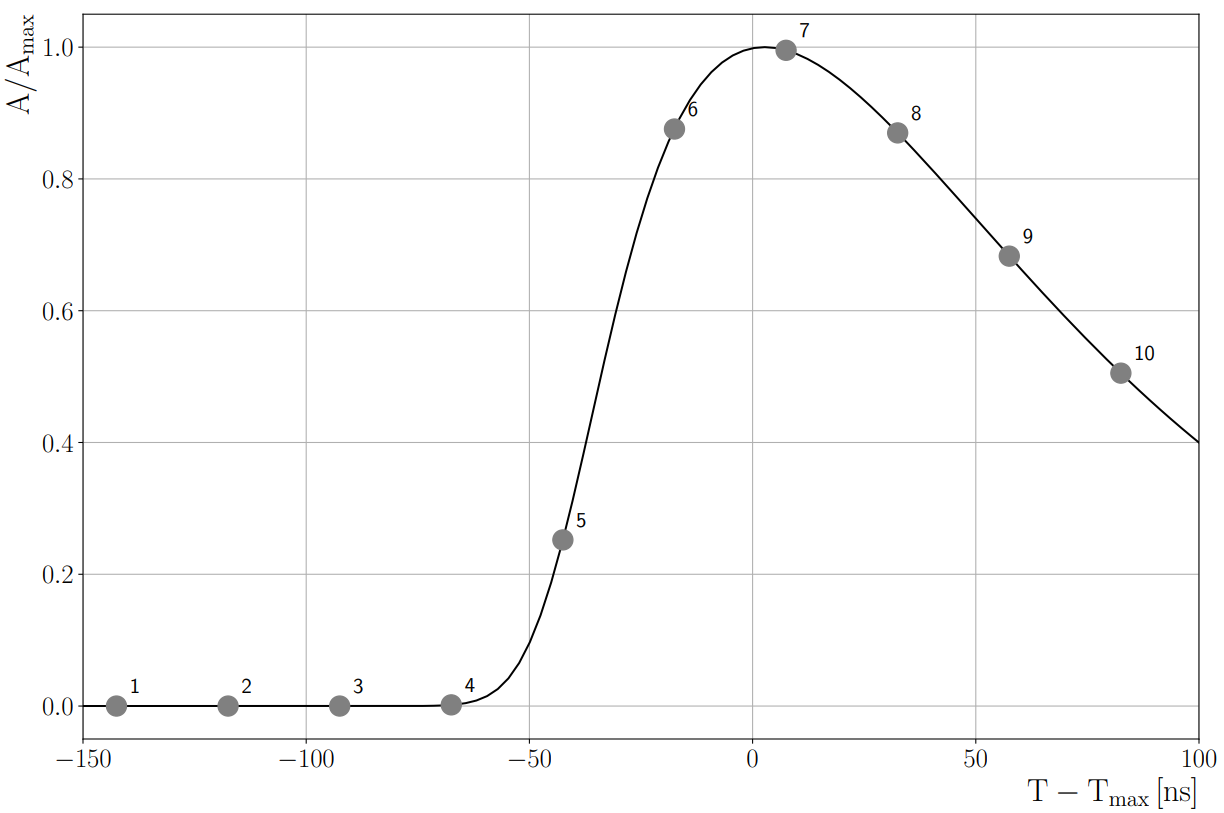
\includegraphics{fig/sec_reco/pulse_template.png}}
\caption{Typical ECAL pulse shape as a function of the difference between the ADC sample time $T$ and the pulse maximum time $T_{\mathrm{max}}$.
The amplitude $A$ is normalized to the maximum pulse amplitude $A_{\mathrm{max}}$.
The solid line shows the expected pulse shape after amplification, while the points indicate the ten discrete samples recorded for a single event, with the pedestal subtracted.}
\label{tec_pulseshape}
\end{center}
\end{figure}

During LHC Run~II (2015--2018), the instantaneous luminosity increased significantly relative to Run~I, resulting in a substantial rise in the number of interactions per bunch crossing (BX).
At the LHC, proton beams are composed of discrete bunches confined in radio-frequency buckets, and a \emph{bunch crossing} corresponds to the moment when two such proton bunches pass through one another at the interaction point.
Each bunch crossing therefore represents a single opportunity for one or more proton--proton interactions to occur and be recorded by the detector.

With the increased luminosity in Run~II, the average number of inelastic proton--proton interactions per BX, referred to as pileup (PU), rose to approximately forty.
These conditions placed significantly more stringent requirements on the ECAL pulse amplitude and time reconstruction, as an increased density of particle interactions contributes energy deposits within a single detector readout window.

In addition, for Run~II the spacing between bunch crossings was reduced from 50\,ns to 25\,ns.
With this reduced spacing, scintillation signals from particles produced in preceding or subsequent bunch crossings can overlap with the signal from the interaction of interest.
Such contributions are referred to as out-of-time pileup (OOT-PU).
As a result, the observed ECAL pulse shape is generally a superposition of an in-time pulse and multiple non-negligible out-of-time pulses originating from both PU and OOT-PU interactions.
This effect is illustrated in Fig.~\ref{tec_multifit2}, where a single OOT pulse is shown for clarity.

To account for the presence of both in-time and out-of-time contributions, a template-based multi-component fit, referred to as the \emph{multi-fit} algorithm, was introduced for ECAL energy reconstruction.
The algorithm estimates the in-time signal amplitude together with amplitudes from up to nine out-of-time contributions by minimizing the $\chi^{2}$ defined as
\begin{equation}
    \chi^{2} = \sum_{i=1}^{N} \frac{\left( \sum_{j=1}^{M} A_{j} p_{ij} - S_{i} \right)^{2}}{\sigma^{2}_{S_{i}}} \, ,
    \label{en-mf}
\end{equation}
where $S_{i}$ denotes the measured amplitude of the $i$th sample, $\sigma^{2}_{S_{i}}$ is the corresponding electronic noise variance, and $p_{ij}$ represents the pulse template for the $j$th bunch crossing contribution evaluated at sample $i$.
The amplitudes $A_{j}$ correspond to the in-time signal and up to $M=10$ out-of-time signals, with templates shifted in time by integer multiples of 25\,ns over a range of $-5$ to $+4$ BXs relative to the in-time interaction.

The pulse templates are derived from low-pileup proton--proton collision data recorded by CMS and are maintained in a periodically updated template library.
The electronic noise term $\sigma^{2}_{S_{i}}$ is determined from dedicated pedestal runs.
The $\chi^{2}$ minimization is performed using a non-negative least-squares technique, enforcing the physical constraint that all fitted amplitudes are positive~\cite{massironi2015precision}.
The reconstructed information associated with a particle interaction in a crystal is referred to as a reconstructed hit (rechit).
The pulse amplitude extracted by the multi-fit algorithm is converted to an energy measurement using calibration constants determined for each crystal.

\begin{figure}[htbp]
\begin{center}
\resizebox{0.75\linewidth}{!}{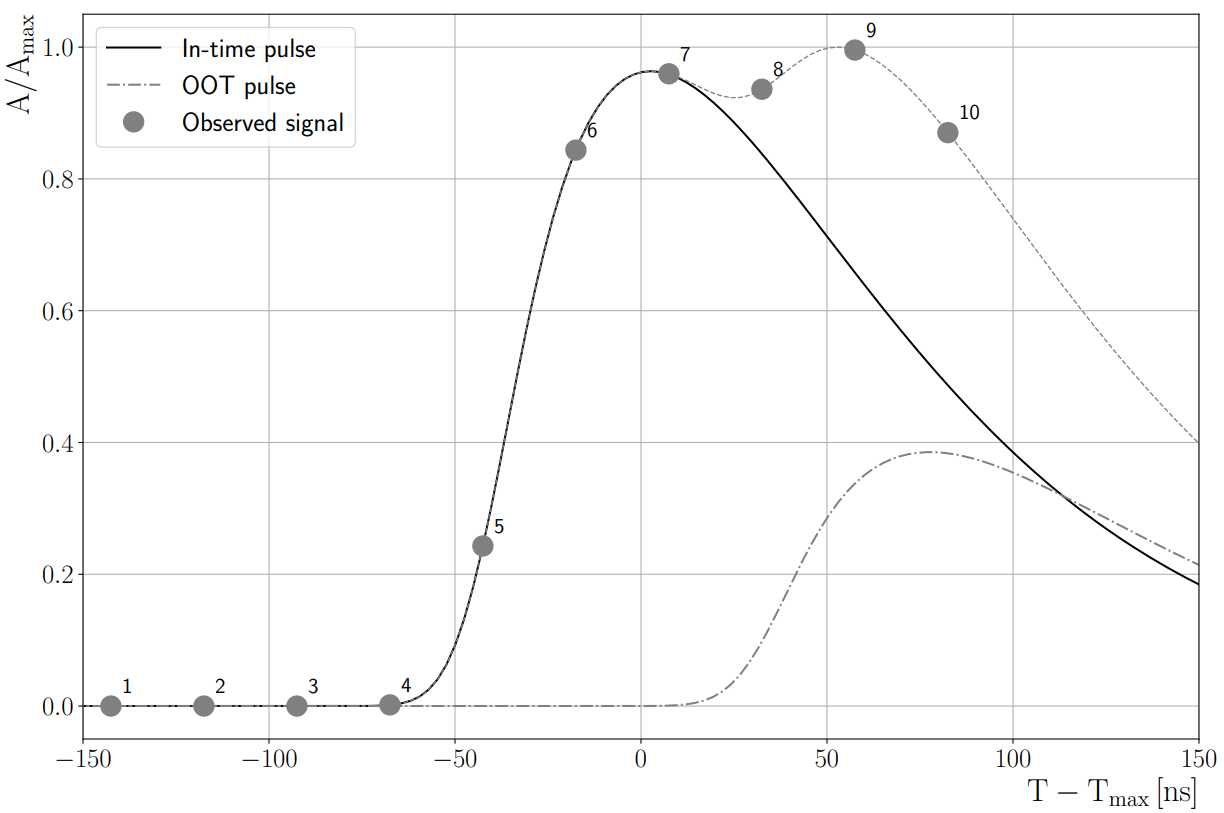
\includegraphics{fig/sec_reco/two_pulses.png}}
\caption{Example of a fitted ECAL pulse for a simulated event with an average of twenty pileup interactions and 25\,ns bunch spacing.
The measured pulse samples (points) are a superposition of an in-time pulse (solid line) and an out-of-time pulse (dashed line).
The amplitude is normalized to the maximum pulse amplitude $A_{\mathrm{max}}$, and the time axis is shown relative to the pulse maximum $T_{\mathrm{max}}$.}
\label{tec_multifit2}
\end{center}
\end{figure}

The ECAL time reconstruction developed for Run~I was used through the beginning of Run~III.
Owing to the fast scintillation response of PbWO$_4$ and the characteristics of the readout electronics, this method achieved time resolutions of order several hundred picoseconds for isolated interactions~\cite{Collaboration_2010}.
Residual channel-to-channel time offsets are corrected using calibration constants derived from data.
The resulting timing information is used, together with topological and energy-based criteria, to reject spurious signals inconsistent with energy deposits from particles produced in proton--proton collisions.
Such signals include direct ionization in the avalanche photodiodes (commonly referred to as spikes), as well as contributions from beam halo muons, cosmic rays, electronic noise, interactions in detector material, and OOT-PU~\cite{CMS-NOTE-2010-012}.

In the original implementation, the arrival time of a rechit was reconstructed by comparing the relative phases of the sampled pulse amplitudes to the expected pulse shape using ratios of consecutive samples.
While effective under the pileup conditions of Run~I, this ratio-based method does not fully account for the increased in-time and out-of-time pileup present in Run~II and Run~III.
The ratio-based time reconstruction algorithm and its limitations are discussed in Section~\ref{sec:algo1}.
To address these challenges, a new cross-correlation (CC) timing reconstruction method was developed during Run~II.
The CC algorithm and its performance are presented in Section~\ref{sec:algo2}.
